% Figure 2: The stationary ray and the corrected constant of the Dollard
% phase: why the modifier must carry (kappa/omega)^{\pm i alpha}.
% Authors: Dr. Davide Batic and Dr. Denys Dutykh
%          (Mathematics Department, Khalifa University of Science and
%           Technology, Abu Dhabi, UAE)
\documentclass[tikz,border=6pt]{standalone}
% ============================================================================
% Shared TikZ style for the figures of the Kerr–Dirac two-channel scattering
% manuscript (compiled standalone into ../latex/figures/).
% Authors: Dr. Davide Batic and Dr. Denys Dutykh
%          (Mathematics Department, Khalifa University of Science and
%           Technology, Abu Dhabi, UAE)
%
% Visual language (used consistently across all figures):
%   * horizon channel      : navy  (chH)
%   * spatial-infinity     : teal  (chI)
%   * accents / emphasis   : gold  (acc)
%   * future/out data      : solid arrows
%   * past/in data         : dashed arrows
%   * proved here          : solid box border
%   * imported input       : light-gray filled box
%   * conditional          : dashed box border
% ============================================================================
\usepackage{amsmath,amssymb}
\usetikzlibrary{arrows.meta,positioning,decorations.pathmorphing,calc,matrix}

\definecolor{chH}{HTML}{142D6E}   % horizon channel (navy)
\definecolor{chI}{HTML}{0E6E6E}   % spatial-infinity channel (teal)
\definecolor{acc}{HTML}{9A7A2E}   % gold accent
\definecolor{warm}{HTML}{9C5310}  % sienna (warnings/exclusions)
\definecolor{ltg}{HTML}{F2F2F2}   % light gray fill (imported)

\tikzset{
  outarr/.style={-{Stealth[length=2.6mm]}, line width=0.9pt},
  inarr/.style={-{Stealth[length=2.6mm]}, line width=0.9pt, dashed},
  axis/.style={-{Stealth[length=2.2mm]}, line width=0.6pt, gray!70!black},
  wavyH/.style={chH, decorate, decoration={snake, amplitude=0.45mm, segment length=2.6mm}},
  wavyI/.style={chI, decorate, decoration={snake, amplitude=0.45mm, segment length=2.6mm}},
  proved/.style={draw, line width=0.7pt, rounded corners=2pt, inner sep=4pt},
  imported/.style={draw=gray!60, fill=ltg, line width=0.5pt, rounded corners=2pt, inner sep=4pt},
  conditional/.style={draw, dashed, line width=0.7pt, rounded corners=2pt, inner sep=4pt},
  lab/.style={font=\small},
  slab/.style={font=\footnotesize},
  tlab/.style={font=\scriptsize},
}

\newcommand{\Log}{\operatorname{Log}} % real odd logarithm of the paper
\begin{document}
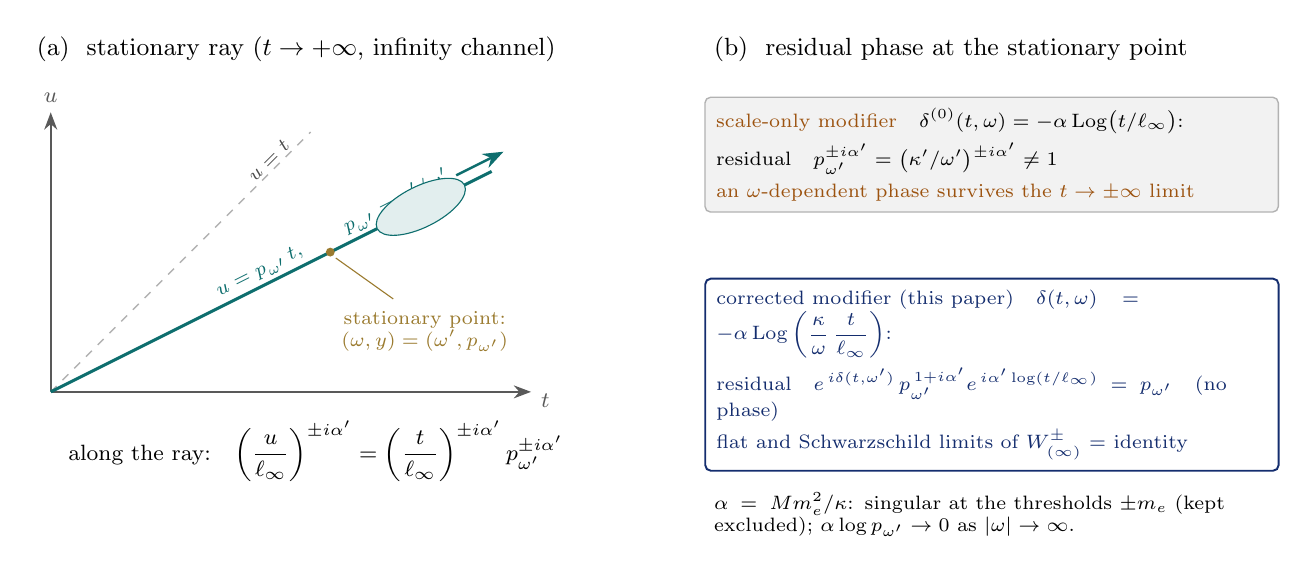
\begin{tikzpicture}[x=1cm,y=1cm]

% ===================== panel (a): the stationary ray ========================
\begin{scope}[shift={(0,0)}]
  \node[lab, anchor=west] at (-0.3,4.35) {(a)\ \ stationary ray ($t\to+\infty$, infinity channel)};
  % axes
  \draw[axis] (0,0) -- (6.1,0) node[slab, anchor=north west, yshift=1mm] {$t$};
  \draw[axis] (0,0) -- (0,3.55) node[slab, anchor=south] {$u$};
  % light ray u = t (reference)
  \draw[gray!60, line width=0.5pt, dashed] (0,0) -- (3.3,3.3);
  \node[tlab, gray!60!black, anchor=west, rotate=45] at (2.45,2.62) {$u=t$};
  % stationary ray u = p t, p = kappa/omega < 1
  \draw[chI, line width=1.1pt] (0,0) -- (5.6,2.80);
  \node[tlab, chI, anchor=west, rotate=26.6] at (2.0,1.22)
    {$u=p_{\omega'}\,t,\qquad p_{\omega'}=\kappa'/\omega'$};
  % wave packet on the ray
  \draw[chI, fill=chI!12, rotate around={26.6:(4.7,2.35)}]
    (4.7,2.35) ellipse (0.62 and 0.26);
  \draw[outarr, chI] (5.15,2.75) -- (5.75,3.05);
  % stationary-point annotation
  \fill[acc] (3.55,1.775) circle (1.6pt);
  \draw[acc, line width=0.4pt] (3.62,1.70) -- (4.35,1.18);
  \node[tlab, acc, anchor=north, align=center] at (4.75,1.15)
    {stationary point:\\ $(\omega,y)=(\omega',p_{\omega'})$};
  % the log identity along the ray
  \node[slab, anchor=west] at (0.1,-0.75)
    {along the ray:\quad
     $\left(\dfrac{u}{\ell_\infty}\right)^{\pm i\alpha'}
      =\left(\dfrac{t}{\ell_\infty}\right)^{\pm i\alpha'} p_{\omega'}^{\pm i\alpha'}$};
\end{scope}

% ===================== panel (b): the two-modifier ledger ===================
\begin{scope}[shift={(8.6,0)}]
  \node[lab, anchor=west] at (-0.3,4.35) {(b)\ \ residual phase at the stationary point};
  \node[imported, tlab, align=left, anchor=north west, text width=7.0cm] at (-0.3,3.75)
    {\textcolor{warm}{scale-only modifier}\quad
     $\delta^{(0)}(t,\omega)=-\alpha\Log\bigl(t/\ell_\infty\bigr)$:\\[0.8mm]
     residual\quad
     $p_{\omega'}^{\pm i\alpha'}=\left(\kappa'/\omega'\right)^{\pm i\alpha'}\neq1$\\[0.8mm]
     \textcolor{warm}{an $\omega$-dependent phase survives the $t\to\pm\infty$ limit}};
  \node[proved, chH, tlab, align=left, anchor=north west, text width=7.0cm] at (-0.3,1.45)
    {\textcolor{chH}{corrected modifier (this paper)}\quad
     $\delta(t,\omega)=-\alpha\Log\left(\dfrac{\kappa}{\omega}\,\dfrac{t}{\ell_\infty}\right)$:\\[0.9mm]
     residual\quad
     $e^{\,i\delta(t,\omega')}\,p_{\omega'}^{\,1+i\alpha'}e^{\,i\alpha'\log(t/\ell_\infty)}
      = p_{\omega'}$\quad(no phase)\\[0.8mm]
     \textcolor{chH}{flat and Schwarzschild limits of $W^\pm_{(\infty)}$ = identity}};
  \node[tlab, anchor=north west, text width=7.0cm] at (-0.3,-1.15)
    {$\alpha=Mm_e^2/\kappa$: singular at the thresholds $\pm m_e$
     (kept excluded); $\alpha\log p_{\omega'}\to0$ as $|\omega|\to\infty$.};
\end{scope}

\end{tikzpicture}
\end{document}
